\documentclass[11pt,a4paper]{article}
\usepackage[spanish]{babel}
\usepackage[utf8]{inputenc}
\usepackage{graphicx}
\usepackage{hyperref}
\usepackage{geometry}
\geometry{a4paper, margin=2.4cm}
\usepackage{mathptmx}
\usepackage{amsmath}
\usepackage{caption}
\usepackage{float}
\usepackage{booktabs}
\usepackage{microtype}
\usepackage{parskip}
\setlength{\parskip}{5pt}

\title{\textbf{Machine Learning II — Deep Learning}\\[4pt]
\large Clasificación automática de imágenes inmobiliarias}
\author{Javier Arroyo García \and Julia Cano Flores \and Paula Durá Fuster}
\date{Abril 2026 · ICAI}

\begin{document}
\maketitle

\section{Introducción y contexto de negocio}

En marketplaces inmobiliarios como Idealista o Zillow, la calidad y la correcta categorización visual de los anuncios influye directamente en la experiencia de los compradores y en la velocidad de venta. La categorización manual de imágenes a escala es costosa, inconsistente y no escalable: un agente inmobiliario puede subir decenas de fotos por propiedad, y clasificarlas correctamente requiere tiempo y criterio especializado.

Este proyecto desarrolla un \textbf{servicio de clasificación automática de imágenes en 15 categorías de escena} orientado a integrarse en el flujo de publicación de un marketplace. El usuario objetivo es el equipo técnico de la plataforma, que necesita una solución robusta, reproducible y con documentación suficiente para operar y mantener en producción. El valor esperado es la reducción del trabajo manual de clasificación y la mejora de la coherencia del catálogo.

Las \textbf{restricciones operativas} del entorno de producción condicionan el diseño del sistema: el servicio debe responder en tiempo real (latencia de inferencia del orden de milisegundos por imagen), debe poder ejecutarse sin GPU dedicada en escenarios de bajo coste (instancias serverless o CPU), y debe ser lo suficientemente preciso como para no requerir revisión manual sistemática.

El pipeline completo está compuesto por tres componentes:
\begin{enumerate}
    \item Selección y comparación de modelos preentrenados mediante transfer learning
    \item Experimentación trazable y búsqueda de hiperparámetros con Weights \& Biases
    \item Despliegue de un servicio de inferencia con FastAPI como backend y Streamlit como interfaz de usuario.
\end{enumerate}

\subsection{Descripción del dataset}

El dataset consta de \textbf{2\,985 imágenes de entrenamiento} y \textbf{1\,500 de validación} repartidas en 15 categorías de escenas interiores y exteriores: \textit{Bedroom, Coast, Forest, Highway, Industrial, Inside city, Kitchen, Living room, Mountain, Office, Open country, Store, Street, Suburb} y \textit{Tall building}. 

\section{Selección de modelos y estrategia de transfer learning}

\subsection{Modelos candidatos}

La elección de modelos se ha hecho intentando cubrir la mayor variedad posible: en lugar de comparar variantes de una misma familia, se seleccionó un representante de cada una de las tres grandes corrientes de la visión por computador moderna. De este modo, los resultados permiten extraer conclusiones sobre enfoques, no solo sobre configuraciones concretas.

\begin{itemize}\setlength\itemsep{2pt}
    \item \textbf{Swin-T} representa los \textit{Vision Transformers}. Su fortaleza reside en comprender el contexto global de una imagen: qué hay a la izquierda, qué hay al fondo, cómo se relacionan las distintas zonas de la escena. Esto lo hace intuitivamente adecuado para imágenes inmobiliarias, donde el conjunto de la habitación importa tanto como sus elementos individuales.
    \item \textbf{ConvNeXt-Small} representa las redes convolucionales modernas. Es la apuesta de mayor capacidad del grupo: incorpora las lecciones aprendidas de los transformadores utilizando la arquitectura convolucional, lo que le permite ser preciso y estable. A priori, es el candidato al mejor rendimiento absoluto.
    \item \textbf{EfficientNetV2-S} representa los modelos orientados a eficiencia. Con menos parámetros y mayor velocidad de inferencia, es el candidato natural para producción en entornos con restricciones de latencia o coste computacional. Se incluye para verificar si la ganancia en precisión de los modelos más grandes justifica su coste adicional.
\end{itemize}

La \textbf{métrica principal} es la \textit{val\_accuracy} (proporción de predicciones correctas en validación), complementada con el \textbf{F1 macro} para detectar sesgos entre clases en un problema de 15 categorías con posible desbalance. Se considera éxito alcanzar $\geq 0.80$ de accuracy con curvas de entrenamiento estables (sin crecimiento sostenido del gap train/val).

\subsection{Estrategia de transfer learning en dos fases}

La idea central del transfer learning es no partir de cero. Los modelos ya han aprendido a reconocer formas, texturas y estructuras visuales en millones de imágenes; el objetivo es reutilizar ese conocimiento y adaptarlo a nuestro problema con el mínimo coste y riesgo posible. Para ello se aplica un esquema de dos fases progresivas, idéntico para los tres modelos.

\textbf{Fase 1 — Aprender a clasificar sin tocar el modelo base (backbone congelado):} en una primera etapa, el cuerpo del modelo se congela por completo y solo se entrena la capa final, que es la única parte nueva. Esta decisión tiene una lógica clara: si se intentara actualizar toda la red desde el principio, los primeros gradientes —procedentes de una cabeza sin entrenar— podrían destruir el conocimiento ya aprendido. Dejar el backbone fijo garantiza un arranque estable y permite que la cabeza se adapte a las 15 clases del problema antes de tocar nada más.

\textbf{Fase 2 — Afinar las capas superiores del modelo (unfreeze de capas):} una vez que la cabeza está orientada al problema, se descongelan los últimos bloques del backbone y se les permite ajustarse también, pero con mucha más cautela. Se usan tasas de aprendizaje distintas para cada parte: más alta para la cabeza (que aún tiene margen de mejora) y mucho más baja para el backbone (para no sobreescribir lo que ya funcionaba bien). El resultado es una adaptación progresiva y controlada al dominio de imágenes inmobiliarias, manteniendo la estabilidad del entrenamiento.

\subsection{Resultados del baseline (fase 1, 8 épocas, AdamW, lr=1e-3)}

\begin{table}[H]
    \centering
    \caption{Resultados del baseline con backbone completamente congelado.}
    \label{tab:baseline-modelos}
    \begin{tabular}{lccccc}
        \toprule
        Modelo & Acc. train & Acc. valid & Loss train & Loss valid & Tiempo/época \\
        \midrule
        Swin-T           & 0.830 & \textbf{0.911} & 0.547 & \textbf{0.275} & 3 min 45 s \\
        ConvNeXt-Small   & 0.766 & 0.855          & 1.016 & 0.881          & 5 min 18 s \\
        EfficientNetV2-S & 0.716 & 0.806          & 0.900 & 0.637          & 3 min 20 s \\
        \bottomrule
    \end{tabular}
\end{table}

Swin-T lidera el baseline con 91.1\% de accuracy y la menor pérdida de validación, lo que indica que sus representaciones preentrenadas son más directamente transferibles a este dominio. Los tres modelos superan ya el criterio de éxito mínimo (80\%) con el backbone congelado, confirmando la calidad de los pesos preentrenados en ImageNet para escenas interiores.

\subsection{Arquitectura de la red desplegada en el API}

Los tres modelos comparten la misma estructura de red en el servicio de inferencia: un \textbf{backbone preentrenado} (ConvNeXt-Small, EfficientNetV2-S o Swin-T según el modelo seleccionado) del que se elimina la cabeza de clasificación original, seguido de una \textbf{capa \texttt{Flatten}} y una \textbf{capa lineal} (\texttt{LazyLinear}) con 15 salidas —una por categoría de escena. La inicialización perezosa de la capa lineal permite reutilizar el mismo código independientemente del tamaño del vector de características de cada backbone. Durante la inferencia, las activaciones de salida se convierten en probabilidades mediante \texttt{softmax} y se devuelven ordenadas por confianza al cliente.

\section{Búsqueda sistemática de hiperparámetros}

\subsection{Diseño experimental y tracking en W\&B}

Para la fase 2 se diseñaron tres sweeps independientes en W\&B, uno por modelo, con \textbf{optimización bayesiana}.
La razón de mantener sweeps separados por modelo, en lugar de un único sweep combinado, es preservar la capacidad comparativa: al tener el mismo presupuesto de ejecuciones para cada arquitectura, ningún modelo queda infrarrepresentado en la búsqueda. Esto permite afirmar que el ranking final refleja el potencial real de cada enfoque bajo una exploración equivalente, y no un sesgo introducido por haber buscado más en unos que en otros.

Se ejecutaron \textbf{12 runs por modelo} (36 en total), con semilla fija (42).

Cada run sigue la convención de nombres \texttt{\{modelo\}\_lr\{lr\_head\}\_wd\{wd\}\_unfreeze\{n\}\_\{optim\}} y se etiqueta con el modelo correspondiente para facilitar el filtrado en W\&B. Por cada run se registraron: \texttt{train/loss}, \texttt{val/loss}, \texttt{val/acc} y \texttt{val/f1\_macro} por época, el tiempo por época, la configuración completa de hiperparámetros y el mejor checkpoint. Al finalizar, se guarda la matriz de confusión sobre el conjunto de validación para el checkpoint restaurado.

El espacio de búsqueda fue el mismo para los tres modelos:

\begin{itemize}\setlength\itemsep{2pt}
    \item \textbf{lr\_head}: log-uniforme en $[10^{-4},\,10^{-2}]$; \quad \textbf{lr\_backbone}: log-uniforme en $[10^{-6},\,10^{-4}]$.
    \item \textbf{optimizer}: AdamW o SGD (momentum 0.9); \quad \textbf{weight\_decay}: $\{0.001,\,0.01,\,0.05,\,0.1\}$.
    \item \textbf{unfreeze\_layers}: $\{0,\,1,\,2,\,3\}$ bloques finales del backbone.
    \item \textbf{warmup\_epochs}: $\{3,\,5\}$; \quad \textbf{finetune\_epochs}: $\{5,\,8,\,10\}$.
\end{itemize}

\subsection{Resultados del sweep}

La Figura~\ref{fig:training-curves} muestra la evolución de la accuracy de validación por época para el mejor run de cada modelo. La Tabla~\ref{tab:sweep-resultados} recoge la mejor configuración encontrada.

\begin{figure}[H]
    \centering
    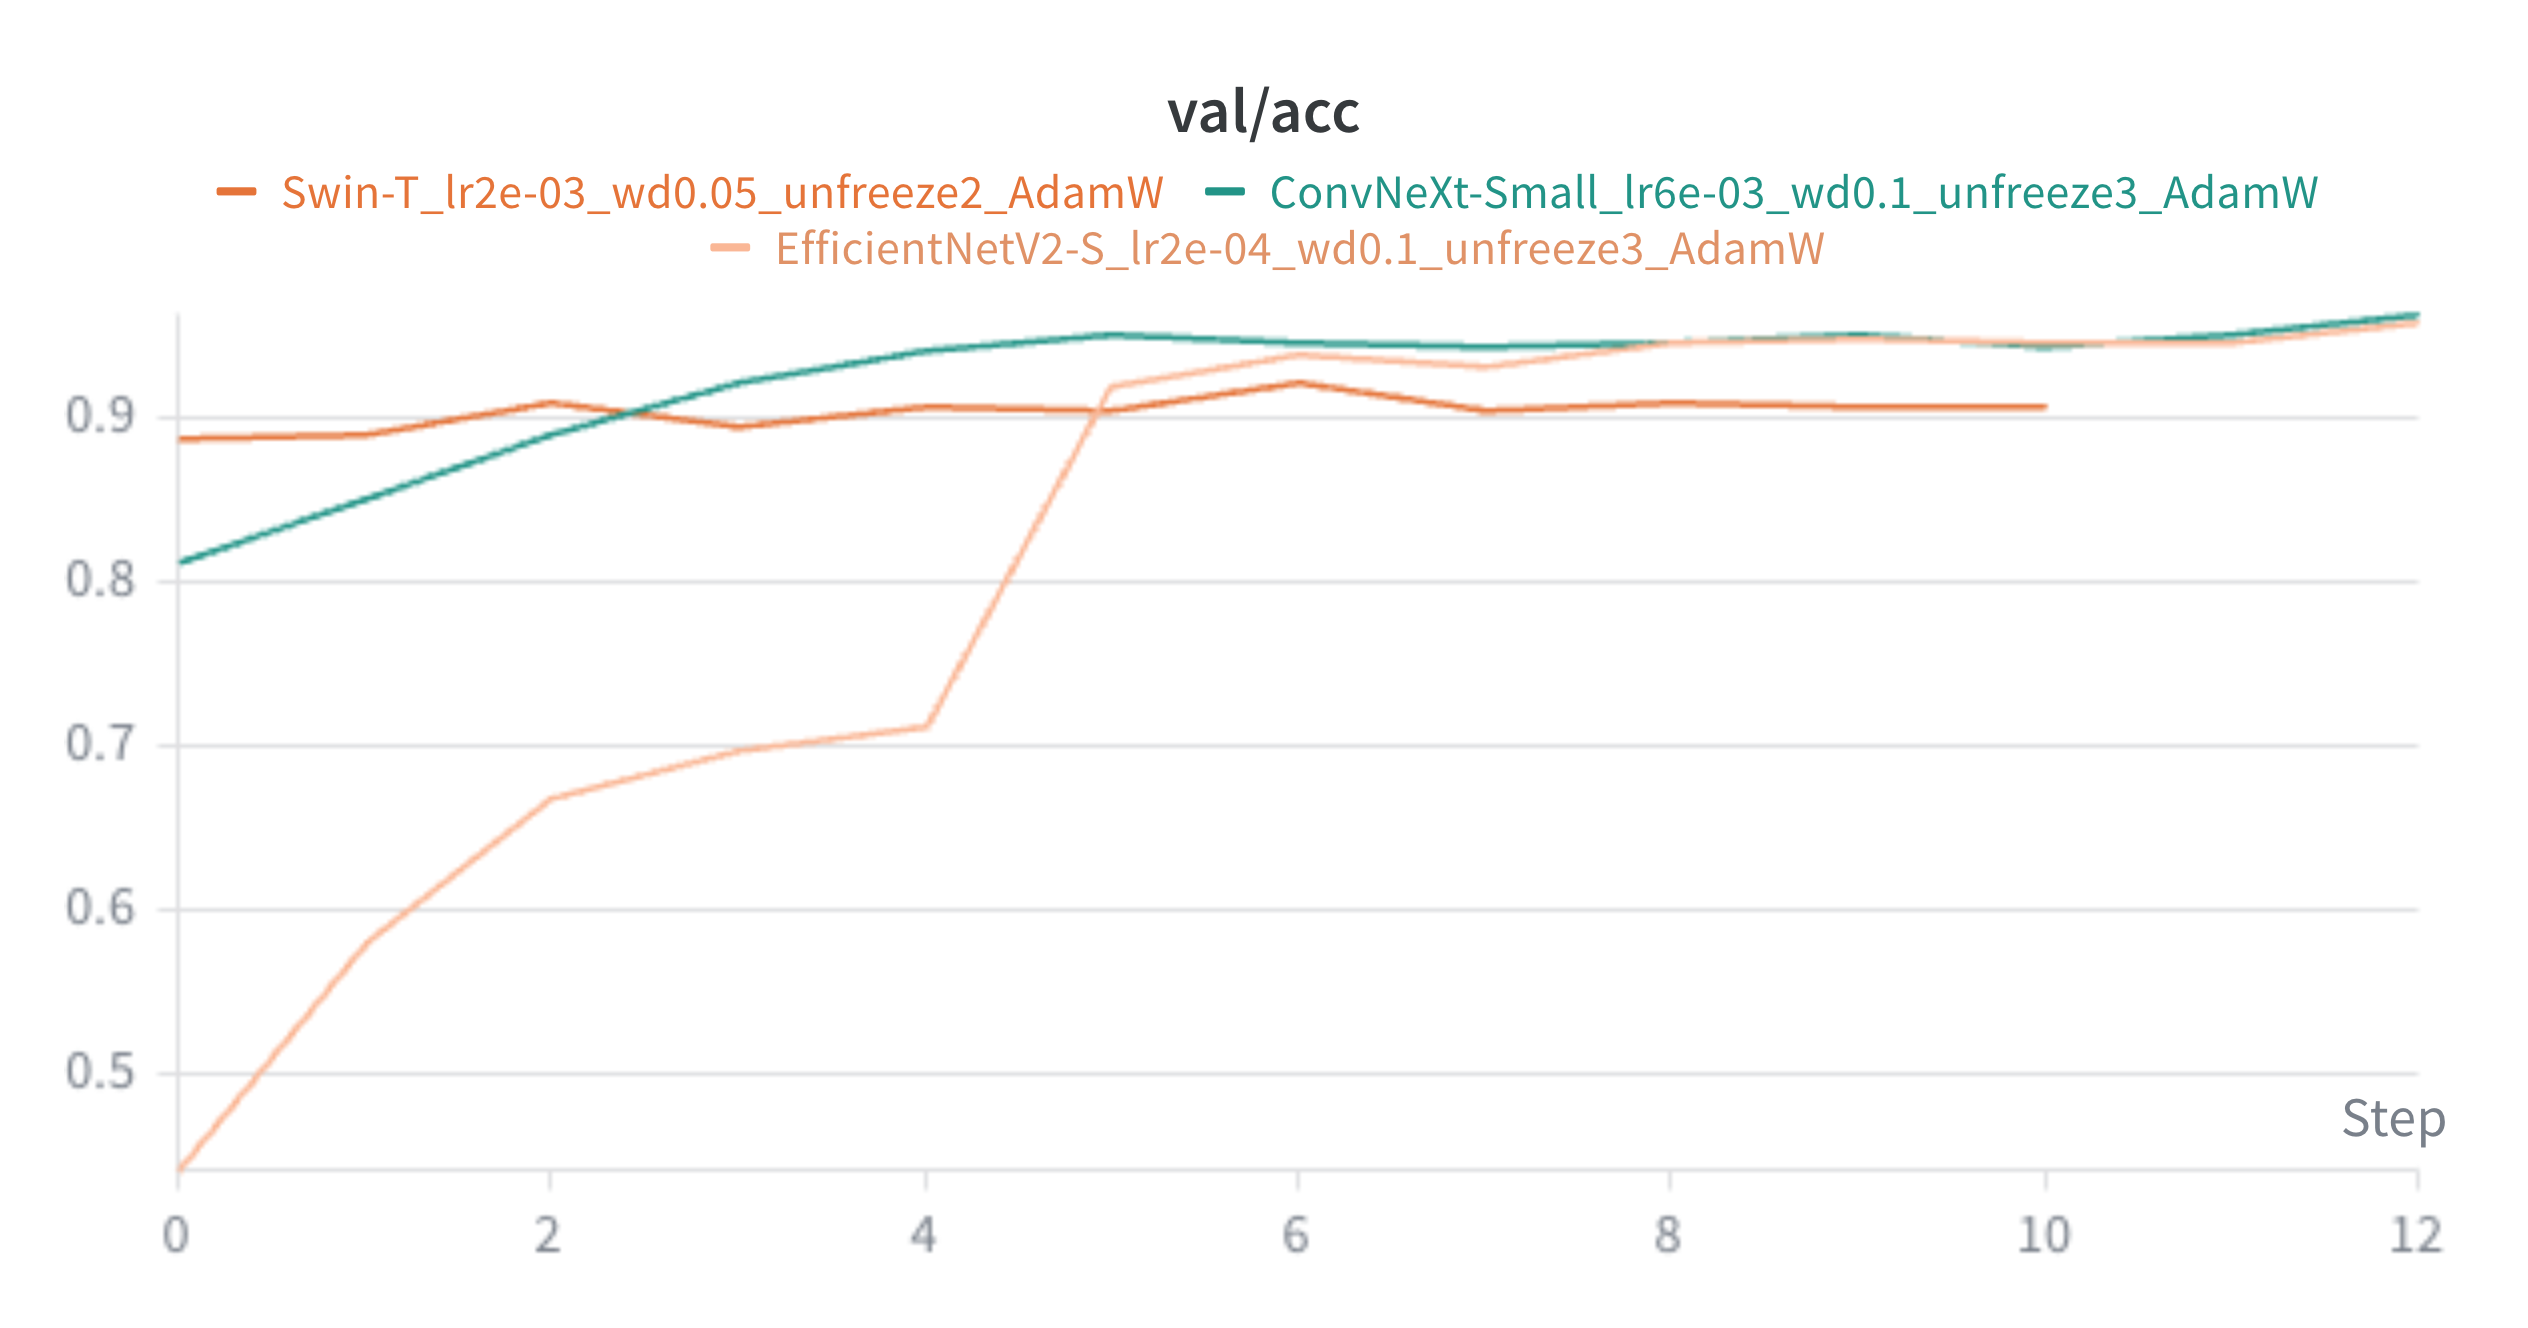
\includegraphics[width=0.82\linewidth]{imagenes/training_curves.png}
    \caption{Curvas de val/acc por época para el mejor run de cada modelo.}
    \label{fig:training-curves}
\end{figure}

La Tabla~\ref{tab:top-runs} muestra los cinco mejores runs por modelo para ilustrar la profundidad de la búsqueda y la estabilidad de las configuraciones ganadoras.

\begin{table}[H]
    \centering
    \caption{Mejor configuración y métricas finales por modelo (36 runs totales).}
    \label{tab:sweep-resultados}
    \begin{tabular}{lcccccc}
        \toprule
        Modelo & Val Acc & F1 Macro & s/época & Optim. & lr\_head & Unfreeze \\
        \midrule
        ConvNeXt-Small    & \textbf{96.47\%} & \textbf{96.47\%} & 99.9 & AdamW & $6.4\!\times\!10^{-3}$ & 3 \\
        EfficientNetV2-S  & 96.00\%          & 96.00\%          & 43.5 & AdamW & $1.8\!\times\!10^{-4}$ & 3 \\
        Swin-T            & 92.27\%          & 92.21\%          & 26.6 & AdamW & $2.4\!\times\!10^{-3}$ & 2 \\
        \bottomrule
    \end{tabular}
\end{table}

\begin{table}[H]
    \centering
    \caption{Top 5 runs por modelo (val\_acc descendente).}
    \label{tab:top-runs}
    \begin{tabular}{llccc}
        \toprule
        Modelo & Configuración & Val Acc & F1 Macro & Optim. \\
        \midrule
        ConvNeXt-S & lr=6.4e-3, wd=0.1, unfreeze=3, ft=10 & 96.47\% & 96.47\% & AdamW \\
                   & lr=6.3e-3, wd=0.1, unfreeze=3, ft=10 & 96.13\% & 96.12\% & AdamW \\
                   & lr=6.0e-3, wd=0.1, unfreeze=3, ft=10 & 95.93\% & 95.93\% & AdamW \\
                   & lr=2.0e-3, wd=0.05, unfreeze=3, ft=10 & 95.87\% & 95.85\% & AdamW \\
                   & lr=1.0e-2, wd=0.05, unfreeze=3, ft=10 & 92.67\% & 92.74\% & SGD   \\
        \midrule
        EffNetV2-S & lr=1.8e-4, wd=0.1, unfreeze=3, ft=8  & 96.00\% & 96.00\% & AdamW \\
                   & lr=5.2e-4, wd=0.1, unfreeze=3, ft=8  & 96.00\% & 96.01\% & AdamW \\
                   & lr=5.1e-4, wd=0.05, unfreeze=3, ft=8 & 95.67\% & 95.67\% & AdamW \\
                   & lr=2.0e-4, wd=0.05, unfreeze=2, ft=5 & 95.07\% & 95.06\% & AdamW \\
                   & lr=2.0e-4, wd=0.05, unfreeze=3, ft=5 & 94.60\% & 94.60\% & AdamW \\
        \midrule
        Swin-T     & lr=2.4e-3, wd=0.05, unfreeze=2, ft=8 & 92.27\% & 92.21\% & AdamW \\
                   & lr=7.9e-3, wd=0.05, unfreeze=2, ft=8 & 92.13\% & 92.12\% & AdamW \\
                   & lr=1.7e-3, wd=0.01, unfreeze=1, ft=5 & 92.13\% & 92.08\% & AdamW \\
                   & lr=2.4e-3, wd=0.05, unfreeze=2, ft=8 & 92.00\% & 91.95\% & AdamW \\
                   & lr=1.2e-3, wd=0.01, unfreeze=1, ft=8 & 92.00\% & 91.94\% & AdamW \\
        \bottomrule
    \end{tabular}
\end{table}

\subsection{Patrones observados}

\textbf{Optimizador:} AdamW dominó en los tres modelos de forma consistente. Los runs con SGD obtuvieron resultados notablemente peores en todos los casos (hasta $-17$ pp en ConvNeXt-Small). La capacidad de AdamW de adaptar la tasa de aprendizaje por parámetro resulta especialmente ventajosa en fine-tuning de redes profundas preentrenadas, donde distintas capas requieren magnitudes de actualización muy diferentes.

\textbf{Capas descongeladas:} \textit{unfreeze=3} fue óptimo para ConvNeXt-Small y EfficientNetV2-S; Swin-T convergió mejor con \textit{unfreeze=2}. Las configuraciones con \textit{unfreeze=0} (solo cabeza, sin fine-tuning) mostraron una caída pronunciada de rendimiento (40--80 pp), confirmando que el fine-tuning parcial del backbone es imprescindible para adaptar las representaciones a nuestro problema.

\textbf{Regularización:} weight\_decay $\geq 0.05$ con AdamW produjo sistemáticamente los mejores modelos, especialmente combinado con learning rates moderados o altos. Una regularización más fuerte controla el sobreajuste que aparece al descongelar capas del backbone con datos de entrenamiento relativamente limitados (2\,985 imágenes).

\textbf{Estabilidad:} Swin-T mostró mayor consistencia entre runs (rango 88\%--92\%), mientras que ConvNeXt-Small y EfficientNetV2-S presentaron mayor varianza ($\sim$15 pp de rango), siendo muy sensibles al optimizador y al número de capas descongeladas.

\textbf{Inversión del ranking:} en el baseline, Swin-T lideraba con 91.1\%. Tras el sweep, ConvNeXt-Small y EfficientNetV2-S lo superan claramente (96\% vs. 92\%), evidenciando que estas arquitecturas tienen mayor capacidad potencial que solo se activa con fine-tuning de capas superiores.

\section{Selección del modelo final y despliegue}

\subsection{Criterio de selección}

\textbf{ConvNeXt-Small} se selecciona como modelo de producción principal por su mayor accuracy (96.47\%) y F1 macro (96.47\%), indicando rendimiento equilibrado en las 15 clases. La diferencia con el baseline de Swin-T (+5.4 pp) y la consistencia de las configuraciones top-4 (todas por encima del 95.8\%) refuerzan la confianza en su generalización.

\textbf{EfficientNetV2-S} constituye la alternativa recomendada cuando se requiere baja latencia: con un 96.00\% de accuracy y $2.3\times$ menor tiempo por época (43.5\,s vs.\ 99.9\,s), es la opción preferible en entornos con restricciones de cómputo, como instancias serverless o despliegues sin GPU.

\subsection{Arquitectura del sistema de inferencia}

El servicio de inferencia en producción está compuesto por dos componentes independientes comunicados a través de HTTP:

\begin{itemize}\setlength\itemsep{3pt}
    \item \textbf{Backend (FastAPI):} expone los siguientes endpoints:
    \begin{itemize}\setlength\itemsep{2pt}
        \item \texttt{GET /} — health check rápido; devuelve \texttt{status} y nombre del modelo cargado.
        \item \texttt{GET /health} — health check detallado; devuelve \texttt{status}, \texttt{model\_loaded} y \texttt{device} (CPU/GPU).
        \item \texttt{GET /classes} — devuelve la lista de las 15 categorías con su índice.
        \item \texttt{GET /model-info} — devuelve metadatos del modelo: arquitectura, ruta del checkpoint, tamaño de entrada, número de clases y dispositivo.
        \item \texttt{POST /predict} — recibe una imagen en base64 y devuelve la clase predicha, la confianza y el nombre de fichero.
        \item \texttt{POST /predict-topk} — recibe una imagen en base64 y el parámetro \texttt{k}; devuelve las \textit{k} clases más probables con sus confidencias, permitiendo al frontend mostrar la distribución completa de predicciones.
    \end{itemize}
    La documentación interactiva (Swagger UI) está disponible en \texttt{/docs} y la estática en \texttt{docs/api.md}.
    \item \textbf{Frontend (Streamlit):} interfaz web que permite cargar imágenes locales o por URL, muestra la predicción principal con su nivel de confianza y visualiza la distribución de probabilidad sobre las 15 clases mediante gráfico de barras interactivo.
\end{itemize}

\subsection{Rendimiento por clase y viabilidad operativa}

Al finalizar cada run, el script registra automáticamente en W\&B la matriz de confusión sobre el conjunto de validación, vinculada al checkpoint y configuración exactos de ese run. Esto permite un análisis de errores trazable y reproducible.

Del análisis de las matrices de confusión se desprenden patrones consistentes: \textit{Highway} y \textit{Suburb} alcanzan el 100\% en los tres modelos, mientras que \textit{Open country} es la clase más difícil (ConvNeXt-Small: 87\%, Swin-T: 75\%), confundiéndose principalmente con \textit{Coast} y \textit{Mountain}. La mayor diferencia entre modelos aparece en clases interiores: Swin-T clasifica \textit{Bedroom} con solo un 78\% (16/100 confundidas con \textit{Living room}), frente al 94\%+ de ConvNeXt-Small y EfficientNetV2-S, lo que explica la brecha de 4~pp en F1 macro.

El F1 macro de 96.47\% de ConvNeXt-Small supera ampliamente el umbral de éxito ($\geq 80\%$) y los errores residuales se concentran en pares de clases ambiguos incluso para un observador humano, lo que los hace aceptables para el caso de uso previsto.

\section{Reproducibilidad}

Los experimentos se ejecutaron en Lightning AI con GPU T4 y entorno Python 3.12 gestionado con conda. El repositorio público incluye:

\begin{itemize}\setlength\itemsep{2pt}
    \item \texttt{requirements.txt} con versiones exactas de todas las dependencias (PyTorch 2.2.1, torchvision 0.17.1, wandb 0.18.1, entre otras).
    \item Semilla global fija (42) aplicada a \texttt{torch}, \texttt{torch.cuda}, \texttt{numpy} y \texttt{random} antes de cada run.
    \item Scripts de entrenamiento (\texttt{sweep\_train.py}) y lanzamiento de sweeps (\texttt{launch\_sweeps.py}) con instrucciones de ejecución en el README.
    \item Checkpoints de los mejores modelos como artefactos versionados en W\&B, accesibles desde el workspace público \texttt{javi\_paula\_julia/image-classification}.
\end{itemize}

\section{Conclusiones y recomendaciones}

El transfer learning sobre arquitecturas modernas preentrenadas permite alcanzar un \textbf{96.47\% de accuracy y F1 macro} en clasificación de imágenes inmobiliarias en 15 clases con tan solo 2\,985 imágenes de entrenamiento y 36 ejecuciones experimentales. Los tres hallazgos principales del proceso de tuning son: (1) AdamW supera a SGD en todos los escenarios de fine-tuning evaluados; (2) descongelar al menos 2--3 bloques del backbone es imprescindible para superar el 92\%; y (3) weight\_decay $\geq 0.05$ mejora consistentemente la generalización cuando se entrena con datos limitados.

\textbf{Recomendación operativa:} desplegar ConvNeXt-Small para máxima precisión, o EfficientNetV2-S cuando la latencia o el coste de inferencia sean críticos. La diferencia de accuracy entre ambos es marginal (0.47 pp), mientras que la diferencia de coste computacional es significativa ($2.3\times$). Para un marketplace con alto volumen de imágenes diarias, EfficientNetV2-S ofrece el mejor balance coste-beneficio.

\textbf{Mejoras futuras:} (1) data augmentation más agresiva (mixup, cutmix) para reducir la varianza y mejorar robustez ante imágenes atípicas; (2) ensemble de ConvNeXt-Small y EfficientNetV2-S por votación suave.

\end{document}
